\chapter{实数、复数与函数}
\label{chap:real-complex-functions}

第~\ref{chap:sets-relations-maps}章的映射可以取值于任意集合，后面研究变化与累计时，取值却几乎总是数。
数之间能够相加相乘，也能比较大小、度量距离；这两类结构分别支撑函数的运算和误差的估计。
实数还有一个有理数没有的性质：有上界的非空集合总有最小上界。
下一章判断极限是否存在，最终都要回到这一点。

本章先整理实数的区间、绝对值与确界原理，再把数扩充到复数，研究复数的运算和平面表示。
随后回到取实数值的函数，区分函数本身、函数的表示和对函数的运算，并讨论有界、单调、对称和最值。
最后复习多项式、指数、对数与三角函数，把数列看作以自然数为输入的函数，整理不需要极限的有限求和。
基本函数这里只作为具体对象使用，它们依赖极限的严格构造和分析性质在后两章给出。

\section{实数}
\label{sec:ru-real-numbers}
\label{sec:real-valued-functions-bounds}

本节沿用读者熟悉的实数及其四则运算和大小关系，整理后文反复使用的两样东西：描述位置与误差的区间和绝对值，以及保证“最小上界”存在的完备性。

\paragraph{区间、绝对值与误差}
在实轴上，区间按端点是否包含分为几种：$[a,b]=\{x:a\leq x\leq b\}$称为闭区间，$(a,b)=\{x:a<x<b\}$称为开区间，$[a,b)$与$(a,b]$称为半开区间。
无界区间写作$[a,+\infty)$、$(-\infty,b)$等，$(-\infty,+\infty)=\mathbb R$。这里的$\pm\infty$只是记号，表示区间在那一侧没有端点，它们不是实数。

数$x$的\term{绝对值}（absolute value）$|x|$在$x\geq0$时等于$x$，否则等于$-x$；$|x-y|$就是实轴上两点之间的距离。
于是$|x-a|<r$恰好表示$x\in(a-r,a+r)$，即$x$落在以$a$为中心、半径为$r$的开区间内。

由$-|x|\leq x\leq|x|$与$-|y|\leq y\leq|y|$相加，得$-(|x|+|y|)\leq x+y\leq|x|+|y|$，即\term{三角不等式}（triangle inequality）
\[
 |x+y|\leq|x|+|y|.
\]
取$x-y$与$y-z$代入，得到$|x-z|\leq|x-y|+|y-z|$：经过第三点绕行，距离不会变短。
把$x=(x-y)+y$代入三角不等式又得$|x|-|y|\leq|x-y|$，交换$x,y$后合并，就是反三角不等式
\[
 \bigl||x|-|y|\bigr|\leq|x-y|.
\]
它说明两数接近时，它们的绝对值也接近。

用$\hat x$近似真值$x$时，$|\hat x-x|$称为\term{绝对误差}（absolute error）。同样的绝对误差对不同大小的真值意义不同：在$1000$上差$1$与在$2$上差$1$，后者严重得多。
因此常用相对误差$|\hat x-x|/|x|$，它把误差与真值的大小比较，所以要求参照值$x\neq0$。例如用$3.14$近似$\pi$，绝对误差小于$0.0016$，相对误差约为$0.05\%$。

\paragraph{确界与确界原理}
\label{sec:ru-supremum-completeness}
集合$A=\{1-1/n:n=1,2,\ldots\}$的元素越来越接近$1$，却没有最大的元素：任一元素$1-1/n$都小于下一个元素$1-1/(n+1)$。
$1$、$2$、$100$都不小于$A$中的每个数，而在这些数中，$1$是最小的一个。下面把这种“最小上界”说清楚。

设$A\subseteq\mathbb R$非空。若$a\leq M$对每个$a\in A$成立，就称$M$为$A$的上界；若$m\leq a$对每个$a\in A$成立，就称$m$为$A$的下界。
存在上界称为上有界，存在下界称为下有界，两者都有称为有界。界不必属于集合，也不唯一。
这正是第~\ref{sec:prelim-order-relations}节偏序集合中上界、下界的定义在$(\mathbb R,\leq)$中的情形。

\begin{definition}[上确界与下确界]
\label{def:ru-supremum}
设$A\subseteq\mathbb R$非空。若$\beta$是$A$的上界，并且任何$A$的上界$M$都满足$\beta\leq M$，就称$\beta$为$A$的\term{上确界}（supremum），记作$\sup A$。
类似地，下界中最大的一个称为\term{下确界}（infimum），记作$\inf A$。
若$\sup A\in A$，就称它为$A$的最大值，记作$\max A$；若$\inf A\in A$，就称它为最小值，记作$\min A$。
\end{definition}

上确界的第二个条件常改写为：对每个$\varepsilon>0$，都存在$a\in A$使$a>\beta-\varepsilon$，即任何比$\beta$小的数都不再是上界。
下确界$\alpha$相应地满足：对每个$\varepsilon>0$，都存在$a\in A$使$a<\alpha+\varepsilon$。

上例中$\sup A=1\notin A$，所以$A$没有最大值；$\inf A=\min A=0$，因为$0=1-1/1\in A$。
可见界、确界与最值是三个层次：界有许多，确界至多一个，最值还要求确界属于集合。

上界有无限多个，其中是否真有最小的一个，并不能从定义看出。本书把下面的性质作为实数的基本性质接受，不加证明。
\begin{theorem}[确界原理]
\label{thm:ru-least-upper-bound}
设$A\subseteq\mathbb R$非空。若$A$上有界，则存在$\beta\in\mathbb R$使$\beta=\sup A$；若$A$下有界，则存在$\alpha\in\mathbb R$使$\alpha=\inf A$。
\end{theorem}
这一性质称为实数的\term{完备性}（completeness），定理本身也称\term{确界原理}（least-upper-bound property）。
关于下确界的一半可由上确界的一半得到：$A$下有界时，$-A=\{-a:a\in A\}$上有界，$-\sup(-A)$就是$\inf A$。

有理数没有这一性质。集合$\{q\in\mathbb Q:q^2<2\}$在有理数中有上界$2$，它在实数中的上确界却是$\sqrt2$，而$\sqrt2$不是有理数。
于是每个有理上界都严格大于$\sqrt2$，在它与$\sqrt2$之间总还有更小的有理上界，有理数中找不到最小的上界。
实数补上了这样的“空隙”。下面三条性质都由确界原理推出，下一章证明极限存在时会直接使用它们。

\paragraph{确界原理的三个推论}
第一个推论说正整数没有上界，这一性质称为\term{Archimedes性}（Archimedean property）。它把“任意大”与“任意小”联系起来，是后面选取尾部起点的依据。
\begin{theorem}[Archimedes性]
\label{thm:ru-archimedean}
对任意实数$x$，存在正整数$n$使$n>x$。等价地，对任意$\varepsilon>0$，存在正整数$n$使$1/n<\varepsilon$。
\end{theorem}
\begin{proof}
若不然，正整数集合以$x$为上界，由确界原理有上确界$s$。$s-1$不是上界，故有正整数$k>s-1$，于是正整数$k+1>s$，与$s$是上界矛盾。
对第二种说法，取$n>1/\varepsilon$即可。
\end{proof}
由此，对每个实数$y$都有唯一的整数$m$满足$m\leq y<m+1$，记作$m=\lfloor y\rfloor$，称为$y$的整数部分：
Archimedes性保证$\{k\in\mathbb Z:k\leq y\}$非空且有上界，它的最大元就是$m$。

第二个推论说有理数在实轴上处处都有。
\begin{theorem}[有理数的稠密性]
\label{thm:ru-rational-density}
对任意实数$a<b$，存在有理数$q$满足$a<q<b$。
\end{theorem}
\begin{proof}
由Archimedes性取正整数$n$使$1/n<b-a$，再令$m=\lfloor na\rfloor+1$，则$m-1\leq na<m$，于是
\[
 a<\frac mn\leq a+\frac1n<b.
\]
取$q=m/n$即可。
\end{proof}
区间无论多短，其中都有有理数；这与第~\ref{chap:cardinality}章证明的“有理数只有可数多个”并不矛盾。

第三个推论把一列逐渐缩小的闭区间压到一点，下一章由它构造收敛子列。
\begin{theorem}[闭区间套定理]
\label{thm:ru-nested-intervals}
设闭区间$[a_1,b_1]\supseteq[a_2,b_2]\supseteq\cdots$逐个嵌套，则存在$c$属于每个$[a_k,b_k]$。
若还对每个$\varepsilon>0$都存在$k$使$b_k-a_k<\varepsilon$，则这样的$c$唯一。
\end{theorem}
\begin{proof}
嵌套使左端点$a_k$单调不减。每个$b_j$都是全部左端点的上界：$k\leq j$时$a_k\leq a_j\leq b_j$，$k>j$时$a_k\leq b_k\leq b_j$。
由确界原理，$c=\sup_ka_k$存在，并且$a_k\leq c$；又因每个$b_k$都是上界，$c\leq b_k$。所以$c$属于每个区间。

若$x<y$都属于每个区间，则每个$k$都有$b_k-a_k\geq y-x>0$，与区间长度可以任意小矛盾。
\end{proof}
定理中的区间必须是闭的：开区间套$(0,1)\supseteq(0,1/2)\supseteq(0,1/3)\supseteq\cdots$没有公共点，因为任何$x>0$都会在$1/k<x$时被排除。
\section{复数}
\label{sec:ru-complex-numbers}

方程$x^2+1=0$在实数范围内没有解，因为实数的平方总不小于零。为了让这类方程也有解，引入一个新的数$i$，规定
\[
 i^2=-1,
\]
并允许它与实数一起按通常的规则相加、相乘。形如$z=a+bi$（$a,b\in\mathbb R$）的数称为\term{复数}（complex number），全体复数记作$\mathbb C$。
$a$称为$z$的实部，记作$\operatorname{Re}z$；$b$称为虚部，记作$\operatorname{Im}z$。两个复数相等，当且仅当实部、虚部分别相等。
$b=0$时$a+0i$就是实数$a$，所以$\mathbb R\subseteq\mathbb C$。下面先确定复数怎样运算，再给出它在平面上的表示。

\subsection{复数的四则运算}
\label{sec:ru-complex-arithmetic}

复数的加减按实部、虚部分别进行：
\[
 (a+bi)\pm(c+di)=(a\pm c)+(b\pm d)i.
\]
乘法先用分配律展开，再把$i^2$换成$-1$：
\[
 (a+bi)(c+di)=ac+adi+bci+bdi^2=(ac-bd)+(ad+bc)i.
\]
可以逐条验证，这样定义的加法与乘法仍满足交换律、结合律和分配律。

除法需要先把分母变成实数。称$\bar z=a-bi$为$z=a+bi$的\term{共轭复数}（complex conjugate），$|z|=\sqrt{a^2+b^2}$为$z$的\term{模}（modulus）。
由乘法公式，
\[
 z\bar z=(a+bi)(a-bi)=a^2+b^2=|z|^2,
\]
它是非负实数，并且只在$z=0$时为零。于是对$w\neq0$，把$z/w$的分子分母同乘$\bar w$，得到
\[
 \frac zw=\frac{z\bar w}{w\bar w}=\frac{z\bar w}{|w|^2}.
\]
右侧的分母是正实数，除法就化成了乘法和实数除法；条件$w\neq0$保证$|w|^2>0$。
共轭与运算相容：$\overline{z+w}=\bar z+\bar w$，$\overline{zw}=\bar z\,\bar w$，逐项展开即可验证。
由此$|zw|^2=zw\,\overline{zw}=(z\bar z)(w\bar w)=|z|^2|w|^2$，即$|zw|=|z|\,|w|$。

复数虽然能做四则运算，却不能像实数那样比较大小。设复数上有一个全序$<$，并与运算相容：$x<y$蕴含$x+z<y+z$，$0<x$与$0<y$蕴含$0<xy$。
那么每个非零数的平方都为正：$x>0$时$x^2=x\cdot x>0$；$x<0$时两边加$-x$得$0<-x$，于是$x^2=(-x)^2>0$。
由此$1=1^2>0$，$-1=i^2>0$，两式相加得$0>0$，矛盾。所以后文的不等式总是比较实数，比如比较复数的模，而不比较复数本身。

\subsection{复数的几何意义}
\label{sec:ru-complex-geometry}

把$z=a+bi$对应到平面上的点$(a,b)$，就得到复数的平面表示，称为\term{复平面}（complex plane）：横轴表示实部，纵轴表示虚部。
由勾股定理，模$|z|=\sqrt{a^2+b^2}$是点$z$到原点的距离，$|z-w|$是两点之间的距离；加法按坐标相加，就是平面上的向量加法，共轭则是关于实轴的反射。
对$z\neq0$，从正实轴到射线$Oz$的转角$\theta$称为$z$的\term{辐角}（argument），它满足
\[
 a=|z|\cos\theta,\qquad b=|z|\sin\theta.
\]
转一整圈回到同一射线，所以辐角只确定到$2\pi$的整数倍：$\theta$与$\theta+2k\pi$（$k\in\mathbb Z$）表示同一个方向。
常取落在$(-\pi,\pi]$中的那个值，称为辐角主值。$z=0$位于原点，没有确定的方向，因而没有辐角。

记$r=|z|$，非零复数可以写成\term{三角形式}
\[
 z=r(\cos\theta+i\sin\theta).
\]
这一写法使乘法有了几何解释。设$z_1=r_1(\cos\theta_1+i\sin\theta_1)$，$z_2=r_2(\cos\theta_2+i\sin\theta_2)$，按乘法公式展开，再用三角函数的加法公式合并实部与虚部，得到
\[
 \begin{aligned}
 z_1z_2&=r_1r_2\bigl[(\cos\theta_1\cos\theta_2-\sin\theta_1\sin\theta_2)+i(\sin\theta_1\cos\theta_2+\cos\theta_1\sin\theta_2)\bigr]\\
 &=r_1r_2\bigl[\cos(\theta_1+\theta_2)+i\sin(\theta_1+\theta_2)\bigr].
 \end{aligned}
\]
所以乘以$z_2$，就是把点$z_1$到原点的距离乘以$r_2$，再绕原点逆时针转过$\theta_2$：模相乘，辐角相加。
例如$i=\cos(\pi/2)+i\sin(\pi/2)$，乘以$i$就是逆时针旋转直角，$i\cdot i=-1$正是把$1$转过两个直角。
图~\ref{fig:ru-complex-multiplication}(a)画出了一个例子。

\begin{figure}[!htbp]
 \centering
 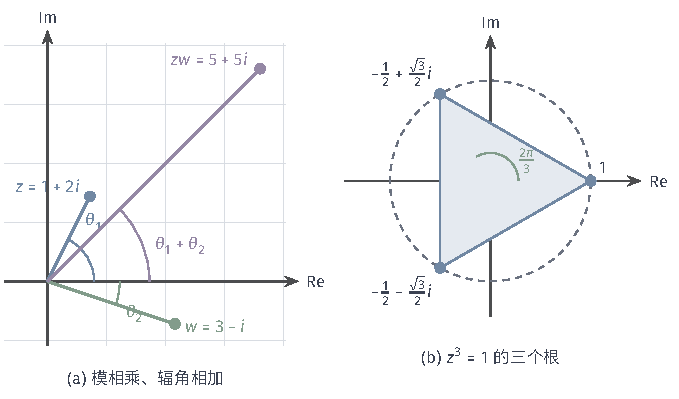
\includegraphics[width=112mm]{figures/01-basic-mathematics/02-real-numbers-and-univariate-functions/tikz/complex-multiplication-roots/figure.pdf}
 \caption{复数乘法与$n$次根的平面表示。(a)蓝、绿两点为$z=1+2i$与$w=3-i$，紫点为乘积$zw=5+5i$。乘积到原点的距离是$\sqrt5\cdot\sqrt{10}$，辐角是两个辐角之和，图中用弧线标出三个辐角。(b)$z^3=1$的三个根$1$与$-\tfrac12\pm\tfrac{\sqrt3}{2}i$都在单位圆上，辐角依次相差$2\pi/3$，构成正三角形的顶点。}
 \label{fig:ru-complex-multiplication}
\end{figure}

反复使用乘法公式并对$n$归纳，得到正整数次幂
\[
 z^n=r^n(\cos n\theta+i\sin n\theta).
\]
由$z\cdot r^{-1}(\cos(-\theta)+i\sin(-\theta))=1$，$z^{-1}$的模为$r^{-1}$、辐角为$-\theta$，所以公式对负整数次幂也成立。

反过来求$n$次根，就是找$w$使$w^n=z$。设$z=r(\cos\theta+i\sin\theta)$，$r>0$，$w=\rho(\cos\varphi+i\sin\varphi)$。
由幂公式，$w^n=z$要求$\rho^n=r$，并且$n\varphi$与$\theta$相差$2\pi$的整数倍。于是$\rho=r^{1/n}$，
\[
 \varphi=\frac{\theta+2k\pi}{n},\qquad k=0,1,\ldots,n-1.
\]
这$n$个辐角互不相差$2\pi$的整数倍，给出$n$个不同的根；$k$取其他整数时只是重复这些根。
它们到原点的距离相同，辐角依次相差$2\pi/n$，恰好是一个正$n$边形的顶点。
例如$z=1$时$r=1$、$\theta=0$，三次根为$1$与$\cos(2\pi/3)\pm i\sin(2\pi/3)=-\tfrac12\pm\tfrac{\sqrt3}2i$，如图~\ref{fig:ru-complex-multiplication}(b)。
三角形式中的$\cos\theta+i\sin\theta$还可以写成指数形式，那需要先用级数定义复指数，留到第~\ref{sec:ru-euler-formula}节。
\section{函数}
\label{sec:ru-functions}

第~\ref{sec:prelim-functions-value-ranges}节的映射可以在任意集合之间建立对应。本节集中考察输入和输出都是实数的映射，
并把三件容易混在一起的事分开：函数本身是什么，函数怎样被写出来，以及怎样由已有函数得到新函数。

\subsection{函数的定义}
\label{sec:ru-function-definition}

设$X\subseteq\mathbb R$。映射$f:X\to\mathbb R$称为实变量的实值\term{函数}（function），$X$是它的\term{定义域}（domain），$\mathbb R$是目标集。
实际取到的值组成像集$f(X)=\{f(x):x\in X\}$，有序对组成的集合$\{(x,f(x)):x\in X\}$称为函数的\term{图像}（graph）。
两个函数相等，要求定义域相同，并且在每个输入处取值相同。
所以同一个表达式配上不同的定义域，就是不同的函数：$x\mapsto x^2$在$\mathbb R$上不是单射，因为$(-1)^2=1^2$；
限制到$[0,+\infty)$上却是单射，后面正是用这种限制构造平方根。

函数可以用公式写出，如$f(x)=x^2$；也可以分段规定，如
\[
 |x|=\begin{cases}x,&x\geq0,\\-x,&x<0.\end{cases}
\]
集合$A\subseteq\mathbb R$的\term{指示函数}（indicator function）$\mathbb I_A$在$A$上取$1$、在其余位置取$0$；
$\mathbb I_{[0,+\infty)}$也写作$\mathbb I\{x\geq0\}$，称为\term{阶跃函数}（step function），它在原点从$0$跳到$1$。
函数还可以由数据表给出，只列出有限个输入处的值。
有限个值不能确定整个函数：$f(x)=x$与$g(x)=x+\sin(\pi x)$在每个整数处取值相同，因为$\sin(k\pi)=0$，
而在$x=1/2$处一个取$1/2$、一个取$3/2$。所以“与数据表一致”只限制了表中的输入，表外的值还需要别的信息。

公式中常同时出现两类字母。在$f(x)=ax+b$中，$x$是输入，取遍定义域；$a,b$在一次讨论中固定，换一组值就换了一个函数。
后一类字母称为参数，把参数取遍某个集合，就得到一族函数。下面用这个例子区分参数、整个函数、输入和函数值。

\paragraph{函数族与参数化}
\label{sec:prelim-function-families}
设想由输入预测输出：事先并不知道哪条规则最合适，通常先划定一批候选规则，再从中挑选。
这批候选规则本身是一个集合，它的元素是整个函数。具有同一定义域和目标集的一组函数组成\term{函数族}（family of functions）。
例如，形如$f(x)=ax+b$的函数称为一元\term{仿射函数}（affine function），所有这样的函数组成
\[
 \mathcal F=\{f_{a,b}:\mathbb R\to\mathbb R:\ f_{a,b}(x)=ax+b,\ (a,b)\in\mathbb R^2\}.
\]
族中的每个元素是一整个函数。取$(a,b)=(2,1)$得到函数$f_{2,1}(x)=2x+1$；再取输入$x=3$，才得到一个函数值$f_{2,1}(3)=7$。

用参数为函数族中的函数编号，称为\term{参数化}（parameterization），一般写成$\theta\mapsto f_\theta$，其中$\theta$属于参数集合$\Theta$。
这个映射的输入是参数，输出是函数；函数$f_\theta$自身的输入仍是$x$。
参数化把“在函数中挑选”改写为“在参数集合中挑选”，参数集合通常是$\mathbb R^2$这样熟悉的集合，便于后续用数值方法比较和调整。

不同参数可能表示同一个函数，所以参数与函数未必一一对应。能否由函数反过来确定参数，取决于下面的条件。
\begin{definition}[函数参数化的可识别性]
\label{def:prelim-identifiable-parameterization}
给定参数集合$\Theta$与函数族$\{f_\theta:X\to Y:\theta\in\Theta\}$。若$f_\theta=f_{\theta'}$蕴含$\theta=\theta'$，即$\theta\mapsto f_\theta$为单射，
则称这一参数化\term{可识别}（identifiable）；否则称为不可识别。
\end{definition}
这里比较的是整个定义域上的函数，而不是几个位置的函数值。仿射函数族中$b=f_{a,b}(0)$、$a=f_{a,b}(1)-f_{a,b}(0)$，
所以完整函数唯一确定$(a,b)$，这一参数化可识别。若只观察$x=0$处的函数值，则只能确定$b$，不能确定$a$。
可见“完整函数能否确定参数”与“有限个观测能否确定参数”是两个不同的问题。

\Needspace{11\baselineskip}
\begin{example}[参数不同而函数相同]
\label{ex:prelim-nonidentifiable-parameterization}
考虑参数化函数
\[
 f_{a,b}:\mathbb R\to\mathbb R,\qquad f_{a,b}(x)=abx,\qquad(a,b)\in\mathbb R^2.
\]
参数$(1,2)$与$(2,1)$不同，却对每个$x$给出相同的函数值。更一般地，只要$c\neq0$，$(ca,b/c)$与$(a,b)$就表示同一个函数。
从完整的输入输出关系可以确定乘积$ab=f_{a,b}(1)$，却不能分别确定$a$和$b$。这是参数化本身不可识别，而不是计算精度不足。
\end{example}

图~\ref{fig:vol1-add-parameter-function-value}把“由参数得到函数”和“由函数得到函数值”这两层操作分开：三组不同参数先汇入同一条完整规则，然后才在指定的$x$处求值。
\begin{figure}[!htb]
 \centering
 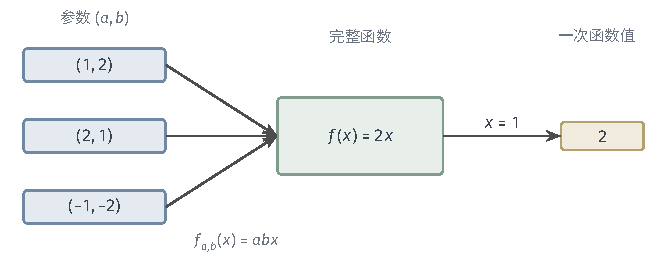
\includegraphics[width=112mm]{figures/00-shared/mathematical-preliminaries-upper/00-shared/tikz/mathematical-language-combinatorics-analysis-optimization-comprehension-additions/parameter-function-value.pdf}
 \caption{参数化$f_{a,b}(x)=abx$中的三层对象。参数$(1,2),(2,1),(-1,-2)$的乘积均为$2$，所以它们表示同一个函数$f(x)=2x$；再指定$x=1$，才得到一次求值结果$2$。多组参数汇入同一完整函数，正是不可识别性。}
 \label{fig:vol1-add-parameter-function-value}
\end{figure}

不可识别的参数可以用第~\ref{sec:prelim-equivalence-relations}节的等价关系整理。规定$\theta\sim\theta'$当且仅当$f_\theta=f_{\theta'}$，
函数相等本身是自反、对称、传递的，所以$\sim$是参数集合上的等价关系。
每个等价类收集同一个函数的全部参数表示；在$f_{a,b}(x)=abx$中，$(a,b)$所在的等价类是满足$a'b'=ab$的全部$(a',b')$。
把每个等价类对应到它所表示的函数，得到商集$\Theta/{\sim}$到函数族的双射；参数化可识别，恰好意味着每个等价类只含一个参数。
统计模型中由有限样本推断参数时的可识别性，留到推断部分讨论。

\subsection{函数的运算}
\label{sec:ru-function-arithmetic}
\label{sec:real-function-arithmetic}

若$f,g:X\to\mathbb R$有相同的定义域，可以在每个输入处对两个函数值做实数运算：
\[
 (f\pm g)(x)=f(x)\pm g(x),\qquad (fg)(x)=f(x)g(x),\qquad (cf)(x)=cf(x),
\]
其中$c$为实常数，这些新函数的定义域仍是$X$。商只在分母不为零的输入上定义：$(f/g)(x)=f(x)/g(x)$的定义域为$\{x\in X:g(x)\neq0\}$。
例如在$\mathbb R$上取$f(x)=x$、$g(x)=x-1$，则$(f+g)(x)=2x-1$定义在整条实轴上，$(f/g)(x)=x/(x-1)$的定义域却不含$1$。
两个函数的定义域不同时，先取公共部分再运算。这些运算都作用在输出值上，与下面的复合不同。

复合把一个函数的输出送入另一个函数作为输入。设$f:X\to\mathbb R$，$g:Y\to\mathbb R$，复合$g\circ f$在$x$处的值是$g(f(x))$，
它只对满足$f(x)\in Y$的$x$有意义。例如$f(x)=1-x^2$、$g(y)=\sqrt y$（$y\geq0$），则$(g\circ f)(x)=\sqrt{1-x^2}$的定义域是$[-1,1]$，
因为只有这些$x$使$1-x^2\geq0$。复合一般不能交换次序：$(f\circ g)(y)=1-y$与$(g\circ f)(x)$是完全不同的函数。

反函数要求先有一一对应。平方函数在$\mathbb R$上不是单射，没有反函数；把定义域限制为$[0,+\infty)$后，它是$[0,+\infty)$到$[0,+\infty)$的双射，
其逆映射就是平方根$y\mapsto\sqrt y$。按第~\ref{sec:prelim-map-operations}节，反函数满足$f^{-1}(f(x))=x$与$f(f^{-1}(y))=y$。
把图像上的每个点$(x,y)$换成$(y,x)$，就得到反函数的图像，即原图像关于直线$y=x$的反射：输入与输出互换了位置。

三个记号需要分清。$f^{-1}$在反函数存在时表示反函数，$1/f$表示逐点取倒数，$f^{-1}(B)=\{x:f(x)\in B\}$表示集合的原像，后者对任何函数都有定义。
以限制在$[0,+\infty)$上的平方函数为例，$f^{-1}(4)=2$，$(1/f)(4)=1/16$；而对定义在$\mathbb R$上的平方函数，原像$f^{-1}(\{4\})=\{-2,2\}$是一个集合，它没有反函数。
\section{函数的性质}
\label{sec:prelim-optimal-values-errors}
\label{sec:ru-function-properties}

从候选函数中挑选时，常把每个候选的优劣写成一个实数，再寻找使它最小的候选。这要求我们能够描述一个函数的取值范围、增减方向和对称性，
并分清“最小的值是多少”和“在哪里取到”。本节把实数集合的确界用到函数的像集上，再用输入之间的关系定义单调、奇偶和周期。

\paragraph{有界性与确界}
设$X$非空，$f:X\to\mathbb R$。函数的有界性就是像集$f(X)$的有界性：若$f(X)$有上界，称$f$上有界，下界与有界同理。
像集的确界简记为
\[
 \sup_{x\in X}f(x)=\sup f(X),\qquad \inf_{x\in X}f(x)=\inf f(X).
\]
若$f(X)$无上界，约定$\sup_Xf=+\infty$；若无下界，约定$\inf_Xf=-\infty$。这两个符号只表示没有有限的界，不是函数实际取到的数。
若存在$x^\star\in X$使$f(x^\star)=\inf_Xf$，就称$f(x^\star)$为$f$的最小值；最大值类似。
例如$f(x)=x$在$(0,1)$上有下确界$0$，却没有最小值：任一允许的输入$x$都有更小的允许输入$x/2$。

\paragraph{单调性}
若对$X$中任意$x<y$都有$f(x)\leq f(y)$，称$f$单调不减；若总有$f(x)<f(y)$，称$f$严格递增。
单调不增与严格递减类似地定义，它们统称\term{单调函数}（monotone function）。单调性比较的是两个输入及其输出的大小关系，与函数能否用公式写出无关。

\paragraph{奇偶性}
奇偶性描述输入取相反数时函数值的变化规律。若定义域关于原点对称（$x\in X$蕴含$-x\in X$），并且$f(-x)=f(x)$，称$f$为偶函数，图像关于纵轴对称；
若$f(-x)=-f(x)$，称$f$为奇函数，图像关于原点对称。定义域不对称时谈不上奇偶：$x^2$在$[0,1]$上不是偶函数，因为$-1/2$不在定义域中。
\paragraph{周期性}
若存在$T>0$，使$x\in X$蕴含$x+T\in X$且$f(x+T)=f(x)$，称$f$以$T$为周期；平移输入$x\mapsto x-c$则把图像整体右移$c$。
这些性质都依赖定义域，讨论时须把定义域与表达式一起写明。

\paragraph{严格单调与反函数}
严格单调还带来可逆性。若$f$在$X$上严格递增，则$x\neq y$时$f(x)\neq f(y)$，$f$是$X$到像集$f(X)$的双射，因而有反函数$f^{-1}:f(X)\to X$。
反函数仍严格递增：若$u<v$属于$f(X)$而$f^{-1}(u)\geq f^{-1}(v)$，两边作用$f$便得$u\geq v$，矛盾。
这里只得到了反函数的存在与单调性；反函数是否连续，要等下一章有了连续性的概念才能讨论。

\paragraph{最小值与最小点}
寻找最小值时，答案包含两部分：最小的函数值是多少，以及哪些输入取到它。若$x^\star\in X$满足
\[
 f(x^\star)\leq f(x)\qquad\text{对所有}\ x\in X,
\]
则称$x^\star$为\term{全局最小点}（global minimizer），$f(x^\star)$为最小值，记作$\min_{x\in X}f(x)$。全部最小点组成的集合记作
\[
 \argmin_{x\in X}f(x)=\{x\in X:\ f(x)\leq f(z)\ \text{对所有}\ z\in X\}.
\]
$\min$给出一个数，$\argmin$给出输入的集合；若不存在最小点，后一个集合为空。
把不等号反向，就得到全局最大点、最大值$\max_{x\in X}f(x)$与集合$\argmax_{x\in X}f(x)$。

最小值存在时必等于下确界：$f(x^\star)$不超过每个函数值，所以是像集的下界；任何下界$m$都满足$m\leq f(x^\star)$，因为$f(x^\star)$本身就是一个函数值。
反过来，下确界存在却未必被取得，前面$(0,1)$上的$f(x)=x$就是例子。
图~\ref{fig:prelim-minimum-infimum}比较同一表达式在$(0,1)$与$[0,1]$上定义的两个函数：区别在于边界点是否属于定义域，而不在于曲线趋向什么高度。

\begin{figure}[htbp]
 \centering
 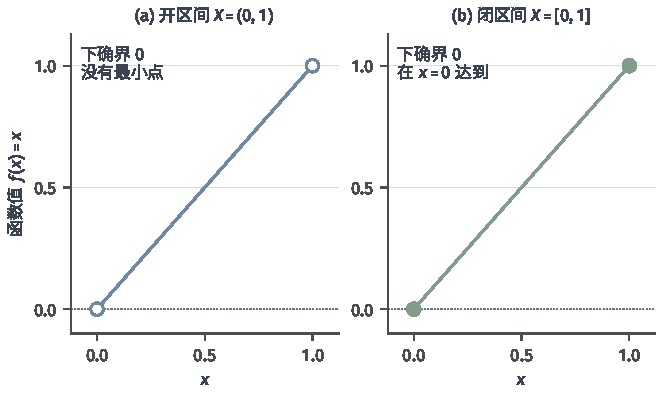
\includegraphics[width=112.0mm]{figures/00-shared/mathematical-preliminaries-upper/01-mathematical-language-combinatorics-analysis-optimization/matplotlib/prelim-minimum-infimum/figure.pdf}
 \caption{同一求值表达式$f(x)=x$在两个定义域上的边界对照。左图定义域为$(0,1)$，空心端点不属于图像，函数值可任意接近$0$，却不能取到；右图定义域为$[0,1]$，实心端点$(0,0)$达到下确界。两图的下确界相同，最小点是否存在取决于可行端点是否保留。图为解析教学示例。}
 \label{fig:prelim-minimum-infimum}
\end{figure}

最小值唯一，最小点却可以有多个。
\begin{example}[同一个最优值可以对应多个输入]
\label{ex:prelim-optimal-value-versus-points}
令$X=[-2,2]$，$f(x)=(x^2-1)^2$。平方非负，且$x=\pm1$都使它为零，所以
\[
 \min_{x\in X}f(x)=\inf_{x\in X}f(x)=0,\qquad \argmin_{x\in X}f(x)=\{-1,1\}.
\]
又因为$0\leq x^2\leq4$，有$|x^2-1|\leq3$，于是$f(x)\leq9$，等号恰在$x=\pm2$处成立，最大值为$9$，最大点集合为$\{-2,2\}$。
\end{example}
例子说明，两个最小点给出的是同一个最小值；最优值相同，并不意味着最优点唯一。怎样求出最小点，是最优化部分的问题，这里只确定它们是什么。
\section{基本函数}
\label{sec:ru-elementary-functions}

后面的例子反复用到几类具体函数：多项式与有理函数、幂函数、指数与对数、三角函数及其反函数。
它们在中学已经出现过，本节只复习怎样辨认它们、它们允许哪些输入，以及常用的恒等式；严格的构造与分析性质留给后两章。

\paragraph{多项式、有理函数与幂函数}
形如$p(x)=c_0+c_1x+\cdots+c_nx^n$的函数称为\term{多项式}（polynomial），它对每个实数$x$都有定义；
两个多项式之商$p(x)/q(x)$称为有理函数，定义域要去掉$q$的零点。幂函数$x^\alpha$的允许输入取决于指数：
正整数次幂对所有$x$有定义；负整数次幂如$x^{-1}=1/x$要求$x\neq0$；$x^{1/2}=\sqrt x$只对$x\geq0$取实数值；
指数$\alpha$不是有理数时，$x^\alpha$只对$x>0$定义，第~\ref{sec:ru-elementary-derivatives}节将用指数和对数给出它的定义。
所以同一个记号$x^\alpha$，定义域会随$\alpha$改变。

\paragraph{指数与对数}
设$a>0$且$a\neq1$。指数函数$a^x$对所有实数$x$有定义，取值恒为正，满足$a^{x+y}=a^xa^y$、$(a^x)^y=a^{xy}$；
$a>1$时它严格递增，$0<a<1$时严格递减。由上一节，严格单调的函数有反函数，指数函数的反函数就是以$a$为底的对数$\log_ax$，定义域为$(0,+\infty)$。
两者互为反函数，意味着$a^{\log_ax}=x$（$x>0$）与$\log_a(a^x)=x$（$x\in\mathbb R$），由此得到$\log_a(xy)=\log_ax+\log_ay$。
底数取$e\approx2.71828$时，$e^x$称为自然指数函数，其反函数记作$\log x$（也记$\ln x$），称为自然对数；本书不加底数的$\log$都指自然对数。
底数为何要求$a>0$：负数的分数次幂可能不是实数，例如$(-1)^{1/2}$；$a=1$时$1^x\equiv1$不是单射，没有反函数。

\paragraph{三角函数与反三角函数}
三角函数通过单位圆定义。从点$(1,0)$出发，沿单位圆逆时针走过弧长$\theta$，到达的点记作$(\cos\theta,\sin\theta)$；
$\theta<0$时顺时针走。用弧长度量角称为弧度制，一周的弧长为$2\pi$。由这一定义，$\cos^2\theta+\sin^2\theta=1$，
正弦和余弦以$2\pi$为周期，正弦是奇函数、余弦是偶函数。正切$\tan\theta=\sin\theta/\cos\theta$要求$\cos\theta\neq0$，即$\theta\neq\pi/2+k\pi$，它以$\pi$为周期。
加法公式
\[
 \sin(\alpha+\beta)=\sin\alpha\cos\beta+\cos\alpha\sin\beta,\qquad
 \cos(\alpha+\beta)=\cos\alpha\cos\beta-\sin\alpha\sin\beta
\]
在复数乘法中已经用过，后面求三角函数的导数时还要用到。

三角函数是周期函数，在整个定义域上不是单射。要得到反函数，须先选一个函数严格单调、并取遍全部函数值的区间。
正弦在$[-\pi/2,\pi/2]$上从$-1$严格增到$1$，它在这一区间上的反函数记作$\arcsin:[-1,1]\to[-\pi/2,\pi/2]$；
余弦在$[0,\pi]$上从$1$严格减到$-1$，相应的反函数为$\arccos:[-1,1]\to[0,\pi]$；正切在$(-\pi/2,\pi/2)$上严格递增，反函数为$\arctan:\mathbb R\to(-\pi/2,\pi/2)$。
例如$\sin(5\pi/6)=1/2$，但$\arcsin(1/2)=\pi/6$，因为$5\pi/6$不在选定的区间内。表~\ref{tab:ru-elementary-functions}汇总这些函数的定义域、值域与周期。

\begin{table}[htbp]
 \centering\small
 \begin{tabular}{@{}llll@{}}
 \toprule
 函数 & 定义域 & 值域 & 周期\\
 \midrule
 $x^n$（$n$为正奇数/偶数） & $\mathbb R$ & $\mathbb R$\,/\,$[0,+\infty)$ & \\
 $x^{-n}$（$n$为正奇数/偶数） & $x\neq0$ & $x\neq0$\,/\,$(0,+\infty)$ & \\
 $\sqrt x$ & $[0,+\infty)$ & $[0,+\infty)$ & \\
 $a^x$（$a>0$，$a\neq1$） & $\mathbb R$ & $(0,+\infty)$ & \\
 $\log_ax$（$a>0$，$a\neq1$） & $(0,+\infty)$ & $\mathbb R$ & \\
 $\sin x$，$\cos x$ & $\mathbb R$ & $[-1,1]$ & $2\pi$\\
 $\tan x$ & $x\neq\pi/2+k\pi$ & $\mathbb R$ & $\pi$\\
 $\arcsin x$ & $[-1,1]$ & $[-\pi/2,\pi/2]$ & \\
 $\arccos x$ & $[-1,1]$ & $[0,\pi]$ & \\
 $\arctan x$ & $\mathbb R$ & $(-\pi/2,\pi/2)$ & \\
 \bottomrule
 \end{tabular}
 \caption{基本函数的定义域、值域与周期。斜线前后分别对应奇数与偶数次幂；$\sqrt x$是平方函数在$[0,+\infty)$上的反函数，$a^x$与$\log_ax$互为反函数。三角函数采用弧度制，$\log$不写底数时指自然对数。}
 \label{tab:ru-elementary-functions}
\end{table}

需要说明这些描述依赖什么。上面把指数函数当作已知对象使用，但“$a^x$对无理数$x$是什么数”“$e$是什么数”都需要极限才能回答；
单位圆上的弧长、$\sin h$与$h$在$h$很小时的比较，也需要极限。
下一章将先用级数构造自然指数函数，由代数和估计得到它的正性、单调性与加法公式，
在介值定理之后严格构造自然对数，并证明三角函数的基本极限；第~\ref{sec:ru-euler-formula}节再由级数得到Euler公式。
在那之前，本节的内容只作为辨认和计算的背景，不用来论证无限求和、连续性或指数与三角函数的关系。
\section{数列与有限求和}
\label{sec:ru-sequences-finite-sums}

数列是以自然数为输入的函数。把它单独列出，是因为下一章的极限首先在数列上定义，而无限求和又要从有限和出发。
本节说明数列与集合、函数族的区别，再推导几类不需要极限的有限和公式。

一个实数\term{数列}（sequence）就是映射$a:\{1,2,\ldots\}\to\mathbb R$，把$n$处的值写作$a_n$，整个数列记作$(a_n)_{n\geq1}$或$(a_n)$；有时下标从$0$开始。
数列记录了每一项的位置，因而与它的取值集合不同：数列$((-1)^n)$在$-1$与$1$之间无限次交替，取值集合$\{-1,1\}$却只有两个元素，次序和重复都看不出来。
数列也不同于函数族：数列的每一项是一个数，函数族的每个元素是一整个函数。下一章研究函数列时，每个编号对应的才是一个函数。

第~\ref{sec:prelim-finite-sums-products}节已经约定了有限和$\sum_{k=1}^na_k$与有限积的记号，这里只回顾三条后面常用的规则。
平移哑索引时范围随之改写，如$\sum_{k=1}^{n}a_{k+1}=\sum_{j=2}^{n+1}a_j$；空和为$0$、空积为$1$，使拆分求和时不必单独处理空的部分；
有限个项的二重和可以交换次序，内层范围依赖外层索引时按式~\eqref{eq:prelim-triangular-sum}重写范围。
交换次序的依据是每个索引对恰好被计入一次，这只对有限多项成立；无限多项的和要先用极限定义，第~\ref{sec:ru-series-rearrangement-grouping}节将看到交换次序可能改变结果。

几类有限和可以直接写出公式。先看$\sum_{k=1}^nk$：把它正着写一遍、倒着写一遍再逐项相加，每一对都等于$n+1$，共$n$对，所以
\[
 \sum_{k=1}^nk=\frac{n(n+1)}2.
\]
由此得到首项为$a$、公差为$d$的等差数列前$n$项之和：
\[
 \sum_{k=0}^{n-1}(a+kd)=na+d\sum_{k=0}^{n-1}k=na+\frac{n(n-1)}2d.
\]
公比为$\rho$的几何和由式~\eqref{eq:prelim-finite-geometric-sum}给出：$\rho\neq1$时$\sum_{k=0}^N\rho^k=(1-\rho^{N+1})/(1-\rho)$，$\rho=1$时为$N+1$。
两个公式都要写清首项、项数和公比；求和从$k=1$开始时，几何和要再乘一个$\rho$。

若每一项能写成相邻两项之差$a_k=b_k-b_{k+1}$，式~\eqref{eq:prelim-telescoping-sum}给出$\sum_{k=1}^Na_k=b_1-b_{N+1}$，中间各项两两抵消，称为裂项求和。
例如$\frac1{k(k+1)}=\frac1k-\frac1{k+1}$，所以
\[
 \sum_{k=1}^N\frac1{k(k+1)}=1-\frac1{N+1}.
\]
这些恒等式对每个固定的$N$成立，只用到有限次运算。当$N$无限增大时，$1-1/(N+1)$与$(1-\rho^{N+1})/(1-\rho)$会怎样变化，下一章用极限回答。

\FloatBarrier
\section{本章小结}
\label{sec:real-complex-functions-summary}

实数部分只做了两件事：用区间和绝对值描述位置与距离，用确界原理保证有界集合有最小上界或最大下界，
并由确界原理得到Archimedes性、有理数的稠密性和闭区间套定理。
复数部分则把$i^2=-1$加入运算，四则运算由实部、虚部逐项计算，除法借助共轭化为实数分母；
在平面上，乘法表现为模相乘、辐角相加。下一章判断极限是否存在时，依靠的是实数的完备性，而不是数值图像。

函数部分区分了函数本身与它的表示：同一表达式在不同定义域上给出不同函数，参数确定函数族中的一个成员，有限个函数值却不能确定整个函数。
最小值是一个数，最小点是输入的集合；下确界存在时，最小值未必存在。
数列是以自然数为输入的函数，有限求和的等差、几何与裂项公式都不需要极限。
到这里为止，误差都是有限步内的数值。项数无限增大、输入无限靠近时会发生什么，是下一章的问题。
